\documentclass[tikz,border=10pt]{standalone}
\usepackage{tikz}
\usetikzlibrary{positioning, fit, calc, shapes.geometric, arrows.meta, backgrounds, patterns}

\begin{document}
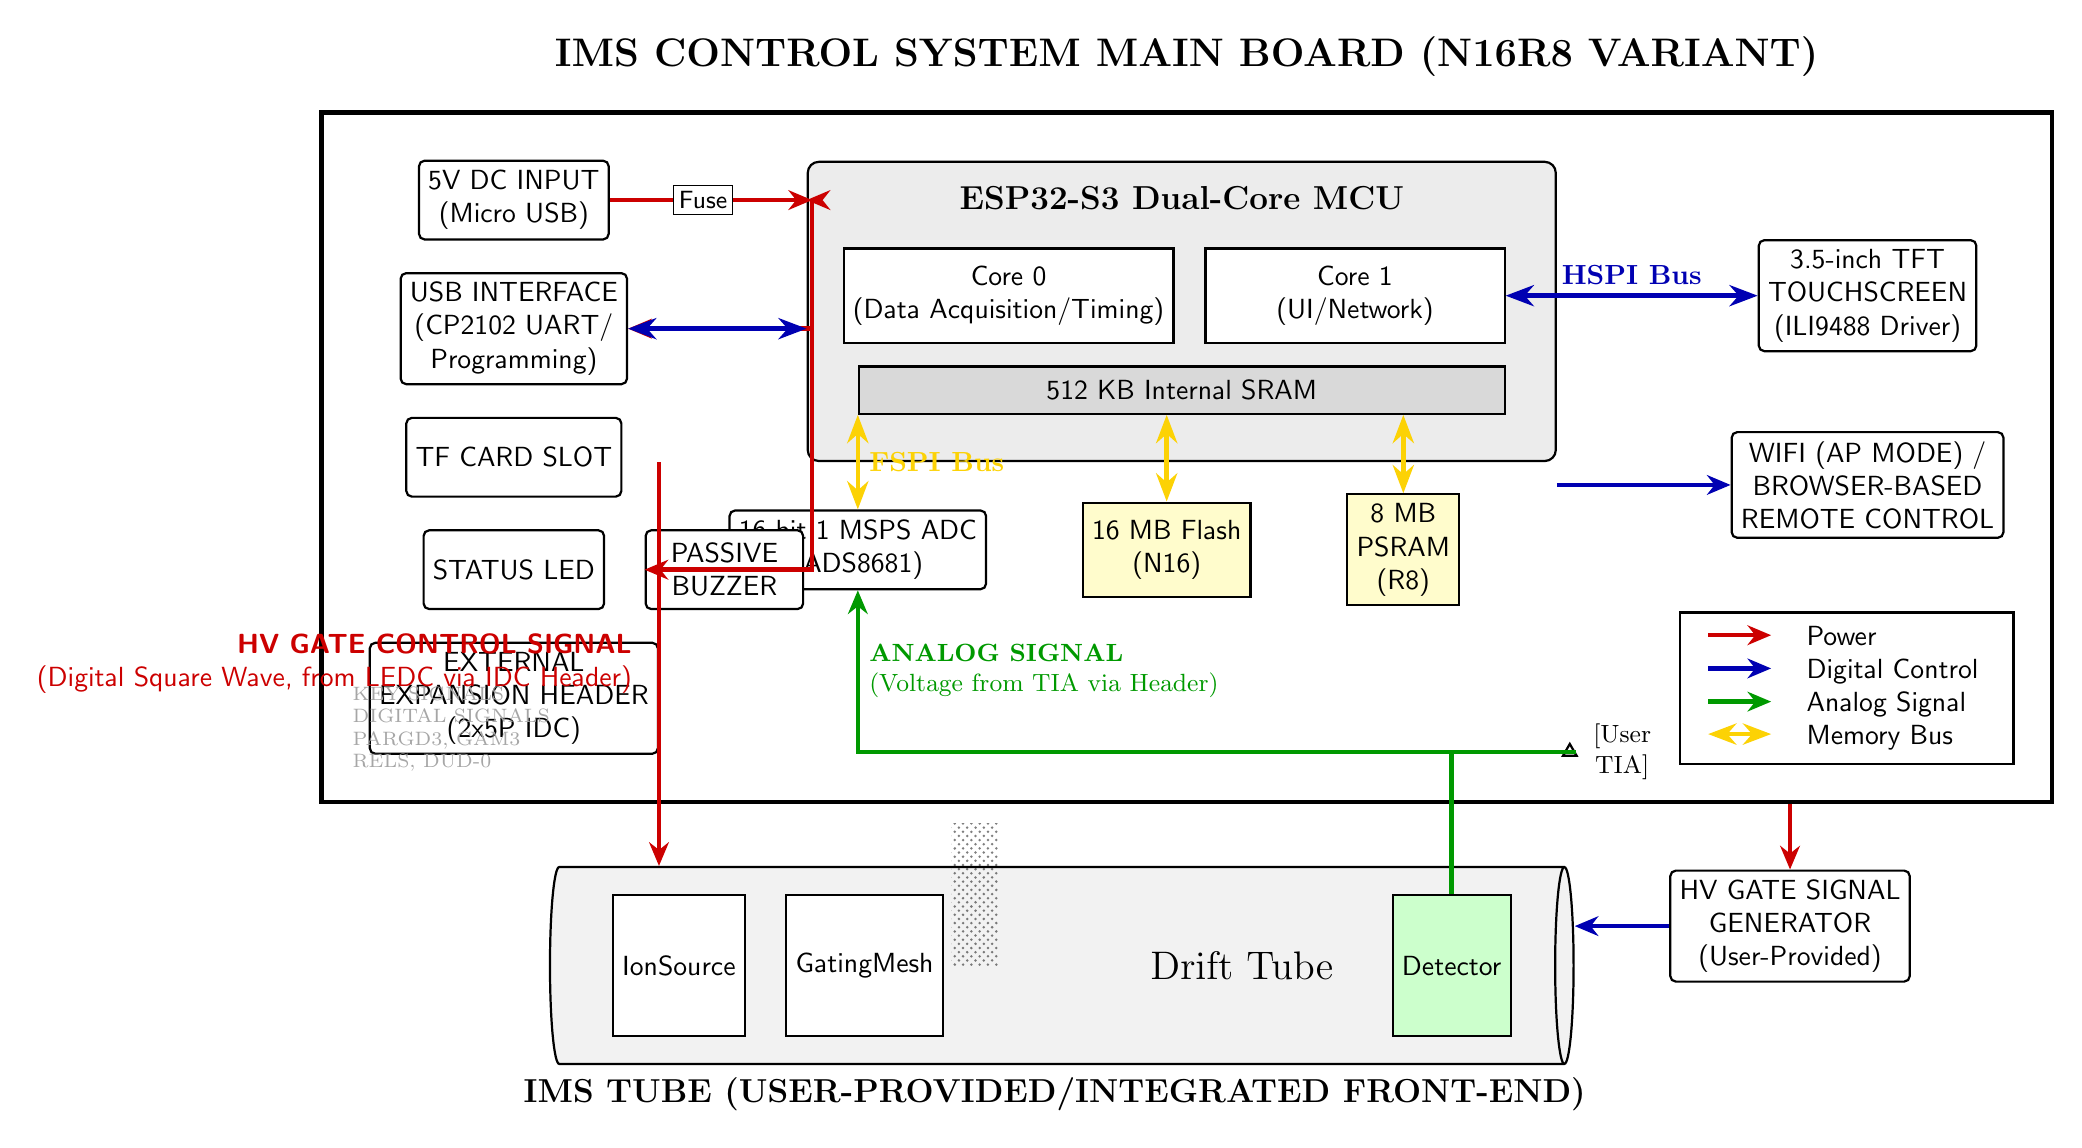
\begin{tikzpicture}[
    >=stealth,
    font=\sffamily,
    % ------------------- 定义全局样式 -------------------
    component/.style={draw, thick, fill=white, align=center, rounded corners=2pt, minimum height=1cm},
    mcu/.style={draw, thick, fill=gray!15, minimum width=9.5cm, minimum height=3.8cm, rounded corners=4pt},
    mcu_core/.style={draw, thick, fill=white, align=center, minimum height=1.2cm, minimum width=3.8cm},
    memory/.style={draw, thick, fill=yellow!20, align=center, minimum height=1.2cm},
    tube/.style={draw, thick, cylinder, shape border rotate=0, minimum height=13cm, minimum width=2.5cm, fill=gray!10},
    % ------------------- 定义线型和颜色 -------------------
    power_line/.style={draw, ultra thick, red!80!black, -{Stealth[length=3mm, width=2.5mm]}},
    digital_line/.style={draw, ultra thick, blue!70!black, -{Stealth[length=3mm, width=2.5mm]}},
    digital_bidir/.style={draw, ultra thick, blue!70!black, <->, >=Stealth},
    analog_line/.style={draw, ultra thick, green!60!black, -{Stealth[length=3mm, width=2.5mm]}},
    mem_line/.style={draw, ultra thick, yellow!70!orange, <->, >=Stealth},
]

% ==================== 1. 主控芯片 (ESP32-S3) ====================
\node[mcu] (mcu_bg) {};
\node[anchor=north, font=\bfseries\large, yshift=-0.2cm] at (mcu_bg.north) {ESP32-S3 Dual-Core MCU};

\node[mcu_core] (core0) at ([xshift=-2.2cm, yshift=0.2cm]mcu_bg.center) {Core 0\\(Data Acquisition/Timing)};
\node[mcu_core] (core1) at ([xshift=2.2cm, yshift=0.2cm]mcu_bg.center) {Core 1\\(UI/Network)};

\node[draw, thick, fill=gray!30, minimum width=8.2cm, minimum height=0.6cm, align=center] 
    (sram) at ([yshift=-1cm]mcu_bg.center) {512 KB Internal SRAM};

% ==================== 2. 底部存储与采集芯片 ====================
\node[component, below=1.2cm of sram.south west, anchor=north] (adc) {16-bit 1 MSPS ADC\\(ADS8681)};
\node[memory, right=1.2cm of adc] (flash) {16 MB Flash\\(N16)};
\node[memory, right=1.2cm of flash] (psram) {8 MB\\PSRAM\\(R8)};

% ==================== 3. 左侧外设 (接口/电源) ====================
\node[component, left=2.5cm of mcu_bg.north west, anchor=east, yshift=-0.5cm] (usb_pwr) {5V DC INPUT\\(Micro USB)};
\node[component, below=0.4cm of usb_pwr] (usb_data) {USB INTERFACE\\(CP2102 UART/\\Programming)};
\node[component, below=0.4cm of usb_data] (tf) {TF CARD SLOT};
\node[component, below=0.4cm of tf] (led) {STATUS LED};
\node[component, below=0.4cm of led] (header) {EXTERNAL\\EXPANSION HEADER\\(2x5P IDC)};

\node[component, right=0.5cm of led, minimum height=1cm, minimum width=2cm] (buzzer) {PASSIVE\\BUZZER};

% ==================== 4. 右侧外设 (屏幕/网络) ====================
\node[component, right=3.2cm of core1.east, anchor=west] (tft) {3.5-inch TFT\\TOUCHSCREEN\\(ILI9488 Driver)};
\node[component, below=1cm of tft] (wifi) {WIFI (AP MODE) /\\BROWSER-BASED\\REMOTE CONTROL};

% ==================== 5. 绘制主板大外框 ====================
\node[draw, ultra thick, fill=none, inner sep=0.6cm, 
      fit=(usb_pwr) (adc) (wifi) (tft) (header) (mcu_bg) (psram), 
      label={[font=\bfseries\Large, yshift=0.3cm]north:IMS CONTROL SYSTEM MAIN BOARD (N16R8 VARIANT)}] 
      (main_board) {};

% 左下角的板载文字修饰
\node[align=left, font=\scriptsize, anchor=south west, text=gray!70] 
    at ([xshift=0.3cm, yshift=0.3cm]main_board.south west) 
    {KEY SIGNALS\\DIGITAL SIGNALS\\PARGD3, GAM3\\RELS, DUD-0};

% ==================== 6. 底部物理结构 (IMS Tube & HV Gen) ====================
\node[tube, below=3.5cm of adc.south, xshift=2.5cm] (tube_bg) {};
\node[anchor=south, font=\bfseries\large] at ([yshift=-0.7cm]tube_bg.south) {IMS TUBE (USER-PROVIDED/INTEGRATED FRONT-END)};

% Tube 内部组件
\node[draw, thick, fill=white, minimum height=1.8cm, right=0.8cm of tube_bg.west] (source) {Ion\\Source};
\node[draw, thick, fill=white, minimum height=1.8cm, right=0.5cm of source] (mesh) {Gating\\Mesh};
% 绘制离子门网格纹理
\fill[pattern=crosshatch dots, pattern color=black, opacity=0.5] ([xshift=0.1cm]mesh.east) rectangle ++(0.6, 1.8) coordinate(mesh_right);
\node[right=2.5cm of mesh, font=\Large] (drift) {Drift Tube};
\node[draw, thick, fill=green!20, minimum height=1.8cm, left=0.8cm of tube_bg.east] (detector) {Detector};

% 右下角的高压发生器
\node[component, right=1.2cm of tube_bg.east, yshift=0.5cm] (generator) {HV GATE SIGNAL\\GENERATOR\\(User-Provided)};

% ==================== 7. 连接线与数据流向 ====================

% 1) 电源连线 (Red)
\coordinate (fuse_start) at ([xshift=0.8cm]usb_pwr.east);
\draw[power_line, -] (usb_pwr.east) -- (fuse_start);
\node[draw, rectangle, fill=white, inner sep=2pt, right=0cm of fuse_start] (fuse) {\small Fuse};
\draw[power_line] (fuse.east) -- ++(1,0) coordinate (pwr_split);
\draw[power_line] (pwr_split) |- (mcu_bg.west |- pwr_split);
\draw[power_line] (pwr_split) |- (usb_data.east);
\draw[power_line] (pwr_split) |- (buzzer.west);

% 2) 内存总线连线 (Yellow)
\draw[mem_line] (sram.south -| adc) -- node[right, font=\bfseries] {FSPI Bus} (adc.north);
\draw[mem_line] (sram.south -| flash) -- (flash.north);
\draw[mem_line] (sram.south -| psram) -- (psram.north);

% 3) 数字控制与通讯连线 (Blue)
\draw[digital_bidir] (core1.east) -- node[above, font=\bfseries] {HSPI Bus} (tft.west |- core1.east);
\draw[digital_line] (mcu_bg.east |- wifi) -- (wifi.west);
\draw[digital_bidir] (usb_data.east) -- (mcu_bg.west |- usb_data.east);

% 4) 模拟信号连线 (Green)
\node[draw, thick, regular polygon, regular polygon sides=3, fill=white, rotate=0, inner sep=1pt] 
    (opamp) at ([xshift=1.5cm, yshift=1.8cm]detector.north) {};
\node[right=0.1cm of opamp, font=\small, align=center] {[User\\TIA]};

\draw[analog_line, -] (detector.north) |- (opamp.west);
\draw[analog_line] (opamp.east) -| node[near end, right, align=left, font=\small] 
    {\textbf{ANALOG SIGNAL}\\(Voltage from TIA via Header)} (adc.south);

% 5) 高压门控触发连线 (Red/Blue)
\coordinate (hv_start) at (mcu_bg.south -| header.east);
\draw[power_line] (hv_start) -- node[left, align=right, xshift=-0.2cm] 
    {\textbf{HV GATE CONTROL SIGNAL}\\(Digital Square Wave, from LEDC via IDC Header)} 
    (hv_start |- tube_bg.north);

\draw[power_line] (main_board.south -| generator) -- (generator.north);
\draw[digital_line] (generator.west) -- (tube_bg.east |- generator.west);

% ==================== 8. 图例 (Legend) ====================
\node[draw, thick, fill=white, anchor=south east, align=left] 
    at ([xshift=-0.5cm, yshift=0.5cm]main_board.south east) {
    \begin{tabular}{cl}
    \tikz{\draw[power_line] (0,0) -- (0.8,0);}   & Power \\
    \tikz{\draw[digital_line] (0,0) -- (0.8,0);} & Digital Control \\
    \tikz{\draw[analog_line] (0,0) -- (0.8,0);}  & Analog Signal \\
    \tikz{\draw[mem_line] (0,0) -- (0.8,0);}     & Memory Bus \\
    \end{tabular}
};

\end{tikzpicture}
\end{document}